\documentclass[12pt]{article}
\usepackage{mathtools}
\usepackage{amssymb}
\usepackage{amsthm}
\usepackage{pgfplots}
\usepackage{polski}
\usepackage[utf8]{inputenc}
\usepackage{geometry}
\usepackage{amsmath}
\usepackage{mnsymbol}
\usepackage{graphicx}
\usepackage{textgreek}
\usepackage{float}
\usepackage{caption}
\begin{document}
\newgeometry{tmargin=2cm,bmargin=2cm,lmargin=2cm,rmargin=2cm}
\tableofcontents \newpage
\section{Cel ćwiczenia}
Celem ćwiczenia było zapoznanie się ze sposobem wyznaczania niepewności pomiarowych w prowadzonych doświadczeniach laboratoryjnych, a także wyznaczenie przyspieszenia ziemskiego (grawitacyjnego) w Krakowie za pomocą wahadła matematycznego. 
\section{Wstęp teorytyczny}
Wahadło matematyczne, inaczej zwane wahadłem prostym , którego przykładowy model przedstawiono na Rys. 1, to układ mechaniczny przyjmujący postać punktu materialnego zawieszonego na cienkiej, nierozciągliwej i nieważkiej nici, którego przeciwległy koniec przymocowany jest do nieruchomej powierzchni.
\begin{figure}[H]
\centering
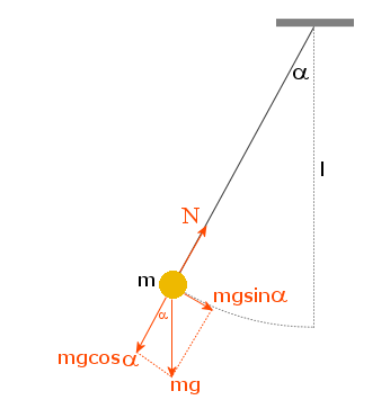
\includegraphics[width=10cm]{1}
\caption*{\textbf{Rys. 1}: Układ wahadła matematycznego z zaznaczonymi siłami działającymi na zawieszone ciało.}
\end{figure}
\noindent Gdy odchylimy takie wahadło o niewielki kąt, który możemy oznaczyć jako α, zawieszony punkt materialny zaczyna drgać z pewnym okresem T. Sytuacja taka możliwa jest jedynie, gdy punkt materialny umieszczony jest w polu grawitacyjnym. Jest to podyktowane tym, że na wychylone ciało musi zadziałać pewna siła, która wprawi go w ruch harmoniczny. Wówczas na podstawie sił działających na wahadło oraz odpowiednich wzorów wiążących ze sobą prawa zachodzące w czasie oscylacji, możliwym jest wyznaczenie wzoru pozwalającego na obliczenie okresu drgań T badanego wahadła. Wzór ten ma następującą postać:
\begin{center}
\LARGE $ T = 2\pi\sqrt{\frac{l}{g}} $
\end{center}
\newpage
\noindent Powyższy wzór wolno stosować jedynie w przypadkach, gdy kąt wychylenia α jest bardzo mały, nieprzekraczający kilku stopni. Wzór ten da się łatwo przekształcić do postaci, dzięki której możliwe jest obliczenie doświadczalne wyznaczenie przyspieszenia grawitacyjnego. Wówczas wzór przybiera postać:
\begin{center}
\LARGE $ g = \frac{4{\pi^2}l}{T^2} $
\end{center}
Doświadczenie składało się z dwóch zasadniczych części. W pierwszej z nich, czterokrotnie cała grupa laboratoryjna zmierzyła czas okresu drgań wahadła matematycznego, przy każdym kolejnym pomiarze wydłużając długość l nitki. Za każdym razem, nie włączano i zatrzymywano stopera dokładnie po jednym cyklu, lecz dopiero po dziesięciu pełnych okresach, a następnie otrzymany wynik podzielono przez tę samą liczbę. Zabieg ten miał na celu zwiększenie dokładności prowadzonego doświadczenia, poprzez zniwelowanie negatywnego wpływu czasu reakcji mierzącego.
W drugiej części doświadczenia obliczyliśmy przyspieszenie grawitacyjne dla każdego z wykonanych pomiarów, wraz z uwzględnieniem jakże istotnych niepewności pomiarowych. Dodatkowo posłużyliśmy się arkuszem kalkulacyjnym za pomocą którego wyznaczono regresję liniową.
\section{Układ pomiarowy}
Wykorzystywany w ćwiczeniach układ pomiarowy składał się z: \newline
1. Zestawu wahadła prostego (w doświadczeniu użyliśmy wahadła fizycznego z zaniedbywalną masą, które potraktowaliśmy jako wahadło proste) (Rys. 2), czyli cienkiej, praktycznie nierozciągliwej nici, o zaniedbywalnej masie oraz metalowego odważnika zawieszonego na tejże nici. \newline
2. Przymiaru milimetrowego (linijka) służącego do pomiaru długości nici. \newline
3. Stopera, dzięki któremu byliśmy w stanie zmierzyć czas trwania 10 okresów. \newline
4. Kalkulatora, za pomocą którego obliczyliśmy przyspieszenie ziemskie.  \newline
\begin{figure}[H]
\centering
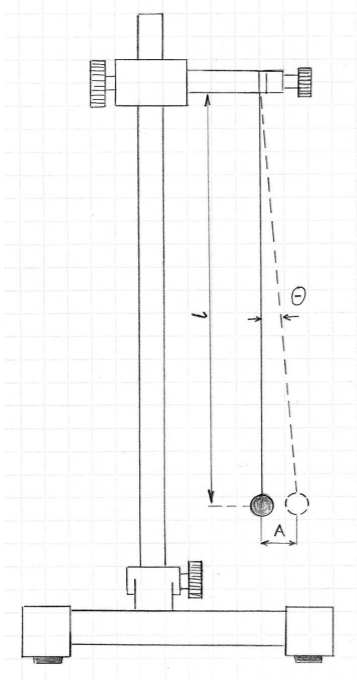
\includegraphics[width=4cm]{2}
\caption*{\textbf{Rys. 2}: Zestaw wahadła prostego}
\end{figure}
\section{Wykonane ćwiczenie}
Doświadczenie rozpoczęliśmy od zmierzenia długości nitki wahadła, od punktu zaczepienia do środka ciężkości, która wyniosła w naszym przypadku l = 13,0 cm. Niepewność pomiaru przyjęliśmy jako sumę niepewności przyrządu oraz niepewności obserwatora. Jako niepewność przyrządu przyjęliśmy działkę elementarną równą 0,1 cm . Zatem u(l) = 0,1 cm. \newline
 W następnym kroku przeszliśmy do mierzenia okresów drgań wahadła, do czego posłużył nam wspomniany wcześniej stoper. Każda osoba z grupy mierzyła okres samodzielnie co zaowocowało 9 różnymi pomiarami okresu drgań $T$. Ćwiczenie powtórzyliśmy jeszcze trzy razy, za każdym razem przyjmując inną długość nitki. Niepewność pomiaru za każdym razem pozostała taka sama.
\section{Wyniki pomiarów}
\begin{figure}[H]
\centering
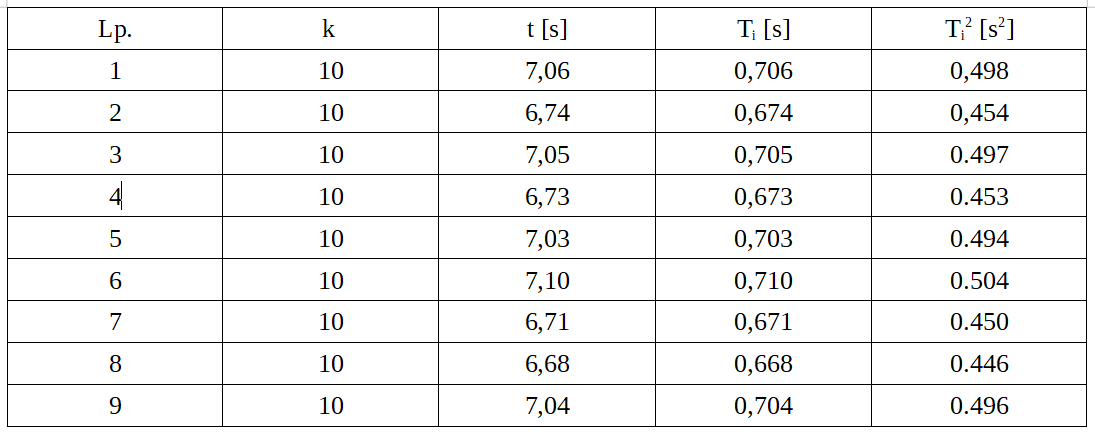
\includegraphics[width=15cm]{3}
\caption*{\textbf{Tab. 1}:	Pomiar okresu drgań dla długości wahadła $l = 13,0$ $cm$, $u(l) = 0,1 $ $cm$ }
\end{figure}
\begin{figure}[H]
\centering
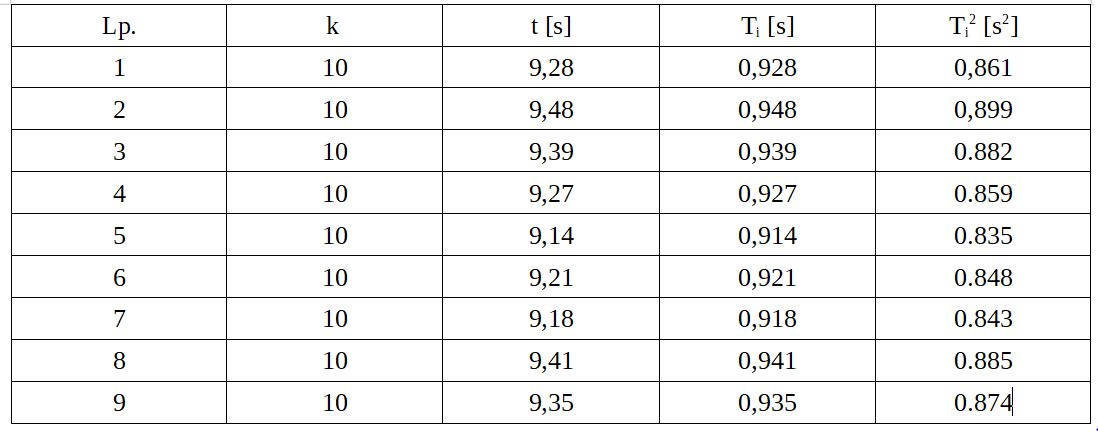
\includegraphics[width=15cm]{4}
\caption*{\textbf{Tab. 2}: Pomiar okresu drgań dla długości wahadła $l = 21,0$ $cm$, $u(l) = 0,1 $ $cm$ }
\end{figure}
\begin{figure}[H]
\centering
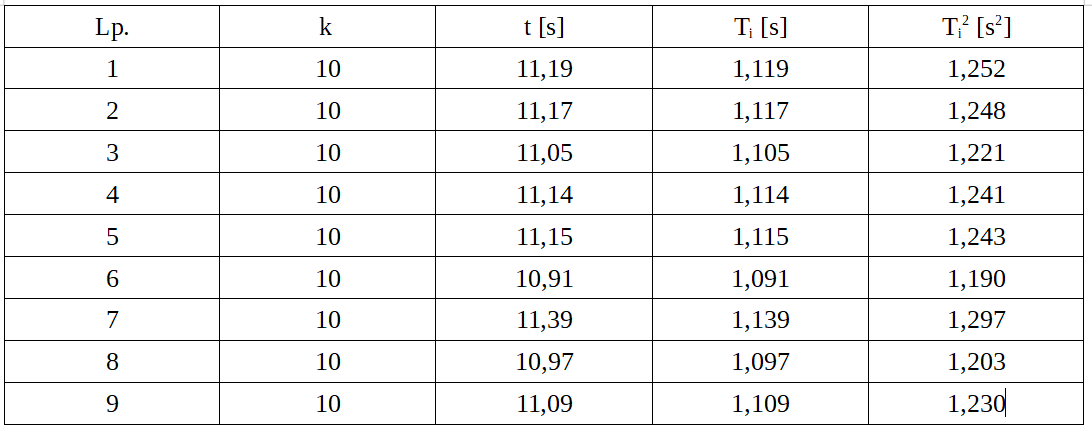
\includegraphics[width=15cm]{5}
\caption*{\textbf{Tab. 3}: Pomiar okresu drgań dla długości wahadła $l = 30,5$ $cm$, $u(l) = 0,1 $ $cm$ }
\end{figure}
\begin{figure}[H]
\centering
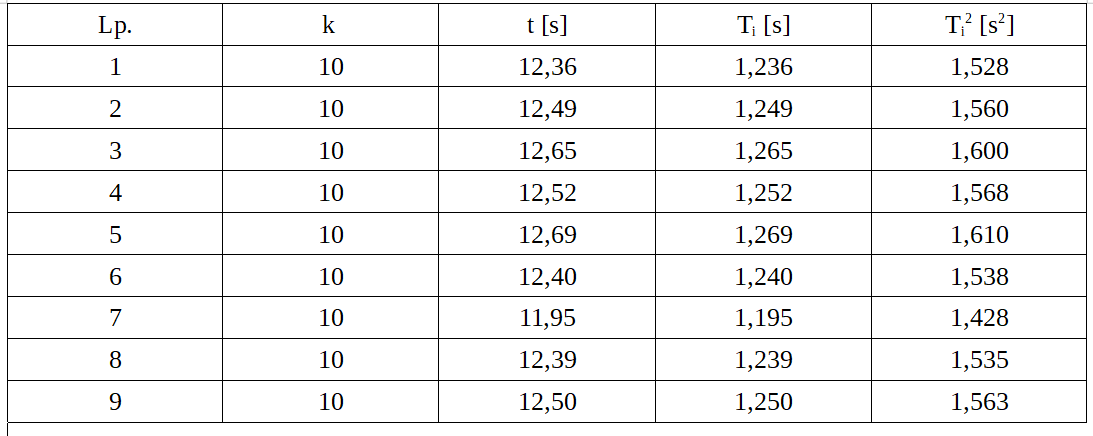
\includegraphics[width=15cm]{6}
\caption*{\textbf{Tab. 4}: Pomiar okresu drgań dla długości wahadła $l = 38,7$ $cm$, $u(l) = 0,1 $ $cm$ }
\end{figure}
\section{Opracowanie wyników pomiaru}
\subsection{Błąd gruby}
Błąd gruby najprawdopodobniej nie wystąpił w żadnym z pomiarów, ponieważ różnica między największym a najmniejszym okresem w każdym z pomiarów 
jest niewielka. Zmierzone wartości wydają się zatem poprawne.
\subsection{Niepewność pomiaru okresu (typu A)}
Niepewność pomiaru okresu typu A, gdzie $T_i$  jest okresem zmierzonym $i$-tym razem dla $n$ pomiarów jest równa:
\begin{center}
\LARGE $ u(T) = \sqrt{\frac{\sum_{i=1}^{n}({T_i}-\bar{T})^2}{n(n-1)}} $
\end{center}
\newpage
Dla danych z Tab. 1:
\begin{center}
\LARGE $ \bar{T} = \frac{\sum_{i=1}^{9}{T_i}}{9} = \frac{6,214}{9} = 0,690 $ $ s $
\end{center}
\begin{center}
\LARGE $ u(T) =  \sqrt{\frac{\sum_{i=1}^{9}({T_i}-\bar{T})^2}{9*8}} = 0,006  $ $ s $
\end{center}
Wartości $u(T)$ dla danych z tabel $2,3,4$ to odpowiednio $0,004$ $s$, $0,005$ $s$, $0,007$ $s$.
\subsection{Niepewność pomiaru długości wahadła (typu B)}
Niepewność pomiaru długości wahadła typu B przyrządu milimetrowego (linijki) wynosi tyle ile działka elementarna, czyli w tym przypadku:
\begin{center}
\LARGE $ u(l) = 1$ $ mm $
\end{center}
\subsection{Przyspieszenie ziemskie}
Po przekształceniu wzoru na długość okresu w wahadle matematycznym otrzymujemy wzór na wartość przyspieszenia ziemskiego: 
\begin{center}
\LARGE $ g = \frac{4{\pi^2}l}{T^2} $
\end{center}
\begin{figure}[H]
\centering
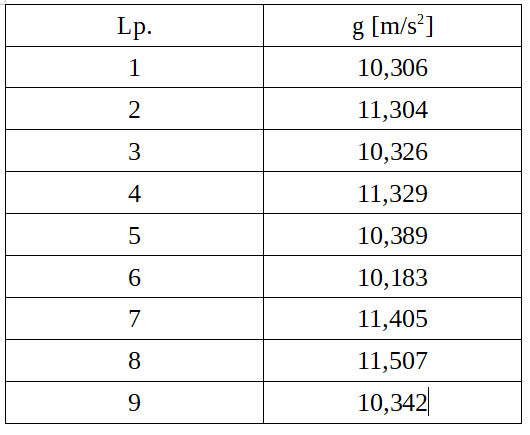
\includegraphics[width=7cm]{7}
\caption*{\textbf{Tab. 5}: Wartości przyspieszenia ziemskiego dla długości wahadła $l = 13,0$ $cm$}
$ g_{sr} = 10,788 $ $m/s^2 $
\end{figure}
\begin{figure}[H]
\centering
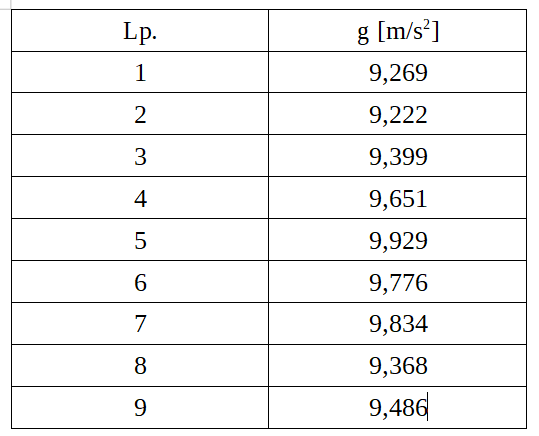
\includegraphics[width=7cm]{8}
\caption*{\textbf{Tab. 6}: Wartości przyspieszenia ziemskiego dla długości wahadła $l = 21,0$ $cm$}
$ g_{sr} = 9,548 $ $m/s^2 $
\end{figure}
\begin{figure}[H]
\centering
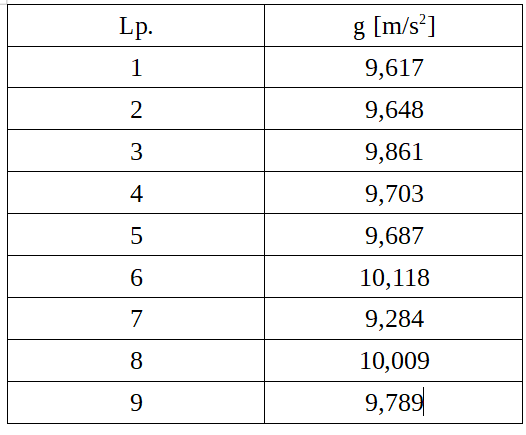
\includegraphics[width=7cm]{9}
\caption*{\textbf{Tab. 7}: Wartości przyspieszenia ziemskiego dla długości wahadła $l = 30,5$ $cm$}
$ g_{sr} = 9,746 $ $m/s^2 $
\end{figure}
\begin{figure}[H]
\centering
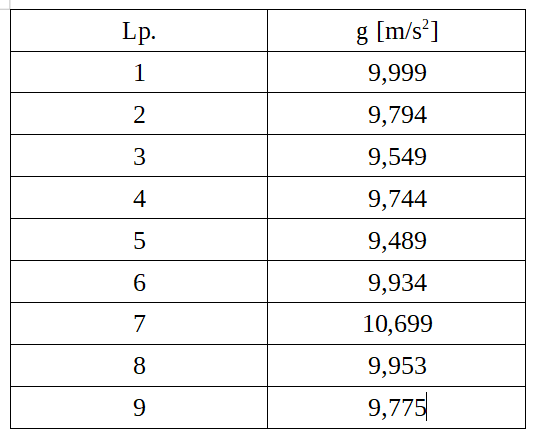
\includegraphics[width=7cm]{10}
\caption*{\textbf{Tab. 8}: Wartości przyspieszenia ziemskiego dla długości wahadła $l = 38,7$ $cm$}
$ g_{sr} = 9,882 $ $m/s^2 $
\end{figure}
\subsection{Niepewność złożona $u(g)$}
Wielkość wynikową g można przedstawić jako funkcję dwóch niezależnych zmiennych (okresu wahadła oraz długości nitki) 
\begin{center}
\LARGE $ g = \frac{4{\pi^2}l}{T^2} $
\end{center}
Wtedy niepewność złożoną możemy przybliżyć przy pomocy prawa przenoszenia niepewności formułą:
\begin{center}
\LARGE $ u(g) = \sqrt{(\frac{\partial{g}}{\partial{l}}u(l))^2+(\frac{\partial{g}}{\partial{T}}u(T))^2}$
\end{center}
Dla danych z Tab. 1:
\begin{center}
\LARGE $ u(g) = \sqrt{(\frac{4\pi^2}{T^2}u(l))^2+(\frac{-8\pi^2l}{T^3}u(T))^2} = \sqrt{(\frac{4\pi^2}{T^2}*1mm)^2+(\frac{-8\pi^2l}{T^3}*0,006s)^2} = 0,205 $ $ m/s^2 $
\end{center}
Pod T podstawiliśmy średnią wartość okresu wahadła z Tab. 1. \newline
Wartości $u(g)$ dla danych z tabel $2,3,4$ to odpowiednio $0,094$ $m/s^2$, $0,068$ $m/s^2$, $0,065$ $m/s^2$.
\subsection{Niepewność rozszerzona $U(g)$}
Przyjmując poziom ufności k = 2 oraz korzystając z danych z Tab. 1, obliczyliśmy niepewność rozszerzoną $U(g)$ korzystając ze wzoru:
\begin{center}
\LARGE $ U_p = k * u_c(g) = 2 * u_c(g) = 0,410 $ $m/s^2  $
\end{center}
Wartości $U(g)$ dla danych z tabel $2,3,4$ to odpowiednio $0,188$ $m/s^2$, $0,136$ $m/s^2$, $0,130$ $m/s^2$.
\subsection{Porównanie obliczonej wartości przyspieszenia ziemskiego z rzeczywistą}
W Krakowie wartość przyspieszenia ziemskiego jest w przybliżeniu równa $9,811$ $m/s^2$. Wyliczone w doświadczeniu wartości średnie wynoszą kolejno $10,788 $ $m/s^2$, $9,548 $ $m/s^2$, $9,746 $ $m/s^2$, $9,882 $ $m/s^2$. Największa różnica wynosi $9,96\%$ zaś najmniejsza $0,66\%$. Widać od razu, że pewne pomiary okazały się dokładniejsze, inne troszkę mniej.
\subsection{Wykres zależności okresu od długości wahadła $T(l)$}
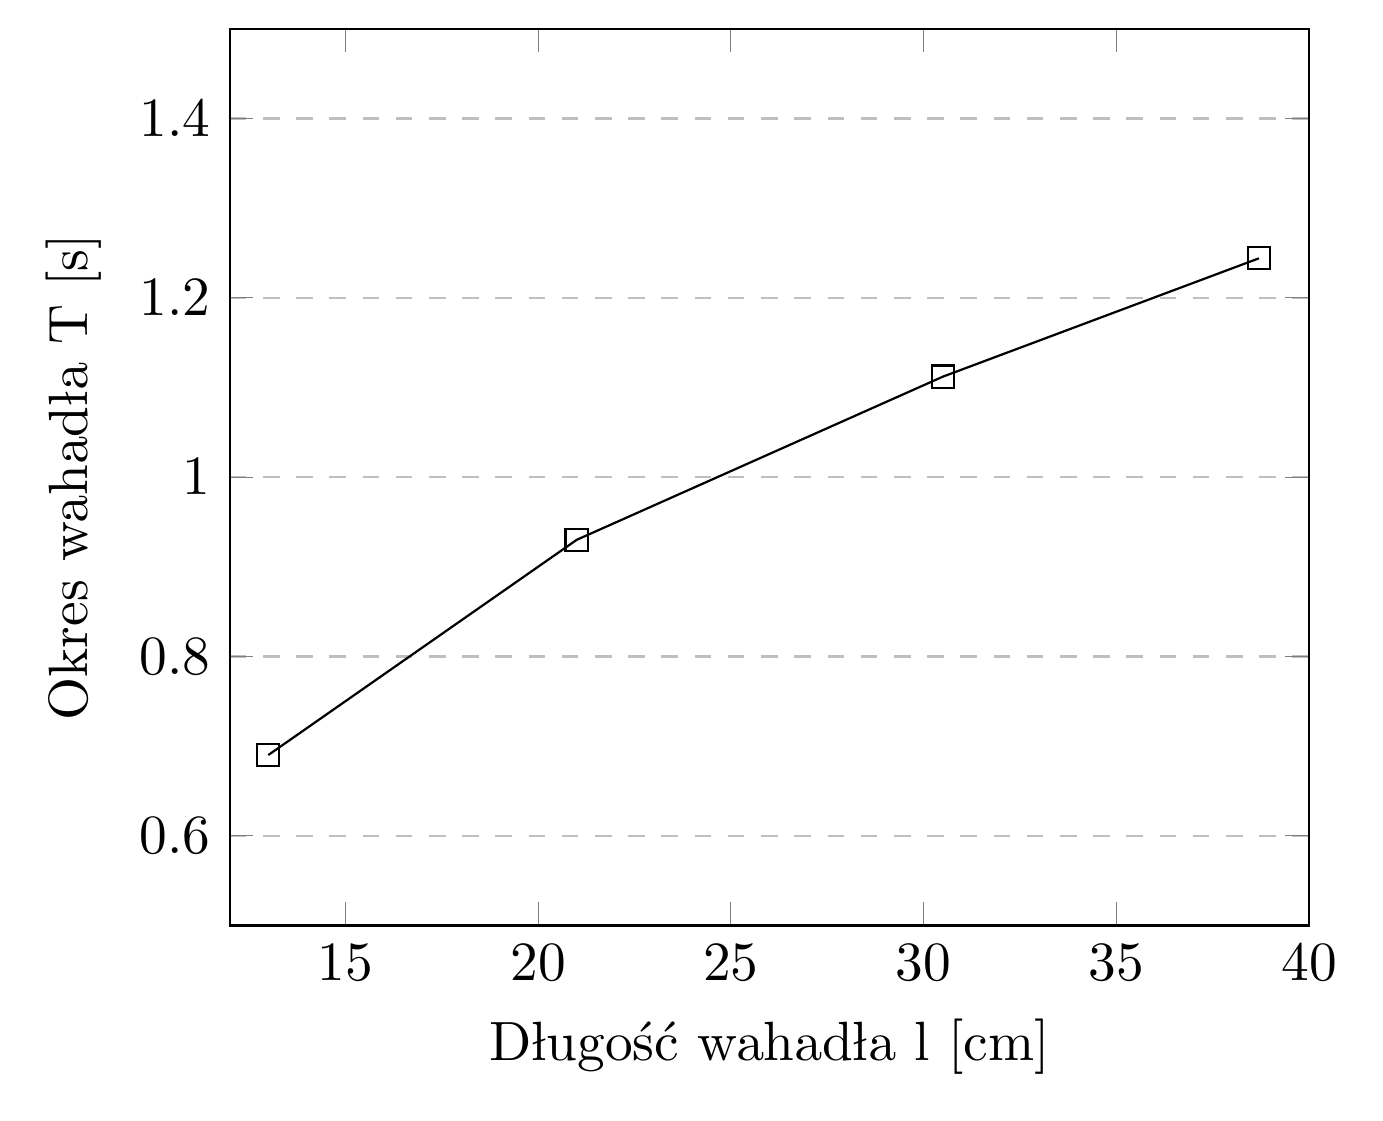
\begin{tikzpicture}[scale=2]
\begin{axis}[
xlabel={Długość wahadła l [cm]},
ylabel={Okres wahadła T [s]},
xmin=12,xmax=40,
ymin=0.5,ymax=1.5,
legend pos=north west,
ymajorgrids=true,grid style=dashed
]

\addplot[color=black,mark=square]
coordinates {
(13,0.690)
(21,0.930)
(30.5,1.112)
(38.7,1.244)
};

\end{axis}
\end{tikzpicture}

\subsection{Wykres zlinearyzowany $T^2$ w funkcji l}
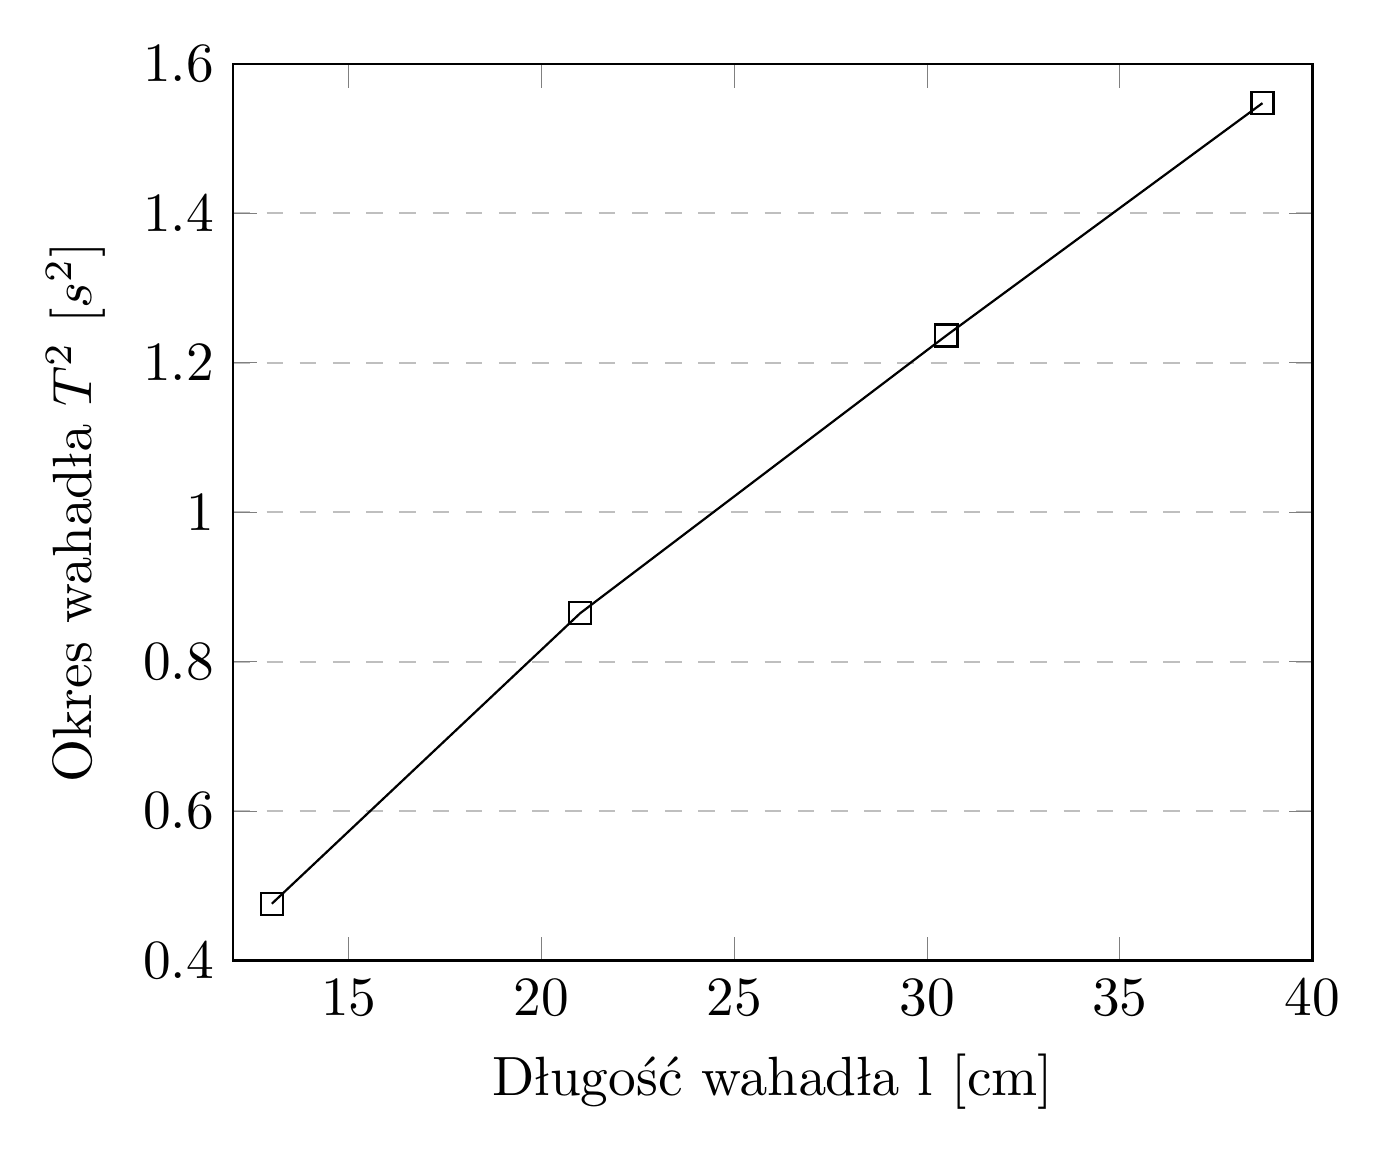
\begin{tikzpicture}[scale=2]
\begin{axis}[
xlabel={Długość wahadła l [cm]},
ylabel={Okres wahadła $T^2$ [$s^2$]},
xmin=12,xmax=40,
ymin=0.4,ymax=1.6,
legend pos=north west,
ymajorgrids=true,grid style=dashed
]

\addplot[color=black,mark=square]
coordinates {
(13,0.4761)
(21,0.8649)
(30.5,1.236544)
(38.7,1.547536)
};

\end{axis}
\end{tikzpicture}

\subsection{Dopasowanie prostej liniowej}
Do znalezienia prostej liniowej dopasowanej do wykresu użyliśmy regresji liniowej. Wspomogliśmy się arkuszem kalkulacyjnym, który wyznaczył nam linię dopasowania: \newline
\begin{center}
\LARGE $ y = 4,137x - 0,036  $
\end{center}
Program wyznaczył również niepewności pomiarowe $ u(a) = 0,168 $ $m/s^2 $ oraz $ u(b) = 0,046 $ $m/s^2 $. \newpage
\subsection{Obliczenie przyspieszenia ziemskiego na podstawie współczynnika nachylenia}
Z równości: $ T^2 = \frac{4\pi^2{l}}{g} $ wynika, że $ a = \frac{4\pi^2}{g} $. Po wyprowadzeniu wzoru na g z tego równania mamy: 
\begin{center}
\LARGE $ g = \frac{4\pi^2}{a} = \frac{4\pi^2}{4,137} $ $m/s^2 = 9,543 $ $m/s^2 $
\end{center} 
\subsection{Niepewność $u(g)$ na podstawie $u(a)$}
Niepewność u(g) możemy obliczyć przy pomocy wzoru na niepewność złożoną: 
\begin{center}
\LARGE $ u(g) = \sqrt{(\frac{\partial{g}}{\partial{a}}*u(a))^2} =|\frac{-4\pi^2}{a^2}*u(a)| = \frac{4\pi^2}{{4,137}^2}*0,168$ $m/s^2 \newline
 = 	0,388$ $m/s^2$
\end{center}
\section{Wnioski}
Po przeprowadzeniu doświadczenia i dokonaniu wszelkich wyliczeń wyciągneliśmy następujące wnioski: \newline
1. Otrzymana wartość przyspieszenia ziemskiego w Krakowie po uwzględnieniu niepewności pomiarowych nie odbiega znacząco od dokładnej wartości przyspieszenia wynoszącej $ 9,81$ $m/s^2$. Wynika z tego, że zarówno pomiary jak i wyliczenia zostały wykonane prawidłowo. \newline
2. Wielokrotne dokonywanie pomiarów, wraz z wydłużeniem okresu wahadła poprzez wydłużenie nitki znacząco poprawiło dokładność pomiarów, co skutkowało dokładniejszym wynikiem końcowym. \newline
3. Dokonywanie pomiaru dla 10 okresów wahadła było doskonałym pomysłem, gdyż znacząco zwiększyło dokładość końcowego wyniku \newline
4. Możliwe jest zwiększenie dokładności wszystkich wyników poprzez zastosowanie dokładniejszych przyrządów, czy też postaranie się na wyeliminowanie w jakiś sposób wpływu czynnika ludzkiego na przeprowadzane doświadczenia, jednak za każdym razem będzie wiązało się to ze znacznym wzrostem kosztów takich pomiarów oraz ich czasochłonności. Na nasze potrzeby otrzymana dokładność w porównaniu z czasem poświęconym na wykonanie doświadczenia jest w zupełności wystarczająca. \newline
5. Lepszym sposobem obliczenia przyspieszenia ziemskiego okazało się użycie regresji liniowej niż skorzystanie z wzoru $ g = \frac{4{\pi^2}l}{T^2} $ oraz oszacowanie niepewności złożonej $u(g)$. Wyniki regresji liniowej pozwoliły obliczyć przyspieszenie ziemskie $g$, które uwzględniając niepewność pomiarową było zgodne z rzeczywistą wartością przyspieszenia. Drugi sposób pozwolił otrzymać taki wynik tylko dla jednego z czterech pomiarów (pomiaru numer 3). Był zatem mniej dokładny, a co za tym idzie, mniej poprawny.                  \newline
6. Arkusz kalkulacyjny w łatwy sposób pozwala nam dopasować prostą do otrzymanych punktów na wykresie. Prosta ta w idealny sposób przechodzi przez 3 punkty odpowiadające za odpowiednio drugi, trzeci i czwarty pomiar. Możemy z tego wywnioskować, że pierwszy pomiar był obarczony największym błędem pomiarowym i najbardziej odbiegał od rzeczywistej wartości przyspieszenia ziemskiego g.
\end{document}